\documentclass{libs/XJTLU_format}
% Inserting the preamble file with the packages
%%%%%%%%%%%%%%%%%%%%%%%%%%%%%%%%%%%%%%%%%%%%%%%%%%%%%%%%%%%%%%%%%%%%%
%% This file contains the packages that can be used in the beamer. %%
%%%%%%%%%%%%%%%%%%%%%%%%%%%%%%%%%%%%%%%%%%%%%%%%%%%%%%%%%%%%%%%%%%%%%
% Package to fonts family
\usepackage[T1]{fontenc}
% Package to accentuation
\usepackage[utf8]{inputenc}
% Package to Figures
\usepackage{graphicx}
% Package to the colors
\usepackage{color}
% Package to the colors
\usepackage{xcolor}
% Packages to math symbols and expressions
\usepackage{amsfonts, amssymb, amsmath}
% Package to multiple lines and columns in table
\usepackage{multirow, array} 
% Package to create pseudo-code
% For more detail of this package: http://linorg.usp.br/CTAN/macros/latex/contrib/algorithm2e/doc/algorithm2e.pdf
\usepackage{algorithm2e}
% Package to insert code
\usepackage{listings} 
\usepackage{keyval}
% Package to justify text
\usepackage[document]{ragged2e}
% Package to manage the bibliography
\usepackage[backend=biber, style=numeric, sorting=none]{biblatex}
% Package to facilities quotations
\usepackage{csquotes}
% Package to use multicols
\usepackage{multicol}
\usepackage{transparent}

% Inserting the references file

\usepackage [spanish]{babel}
\usepackage [utf 8]{inputenc}

% Title
\title[Curso Análisis exploratorio de datos en Python y R]{\huge\textbf{Curso Análisis exploratorio de datos en Python y R}}
% Subtitle
\subtitle{Interfaz de los programas}
% Author of the presentation
\author{Juan Camilo Perdomo}
% Institute's Name
\institute[Universidad del Rosario]{
    % email for contact
    \normalsize{\email{juan.perdomor@urosario.edu.co}}
    \newline
    % University name
    \university{Universidad del Rosario}
    \newline
    % Department Name
    \department{Bogotá, Colombia}
}
% date of the presentation
\date{\today}

%%%%%%%%%%%%%%%%%%%%%%%%%%%%%%%%%%%%%%%%%%%%%%%%%%%%%%%%%%%%%%%%%%%%%%%%%%%%%%%%%%
\begin{document}
% insert the code style
%%%%%%%%%%%%%%%%%%%%%%%%%%%%%%%%%%%%%%%%%%%%%%%%%%%%%%%%%%%%%%%%%%%%%%%%%%%%%%%%%%%
%% This file contains the style of the codes show in slides.                     %%
%% The package used is listings, but it possible to used others.                 %%
%%%%%%%%%%%%%%%%%%%%%%%%%%%%%%%%%%%%%%%%%%%%%%%%%%%%%%%%%%%%%%%%%%%%%%%%%%%%%%%%%%%

% color used in the code style
\definecolor{codegreen}{rgb}{0,0.6,0}
\definecolor{codegray}{rgb}{0.5,0.5,0.5}
\definecolor{codepurple}{rgb}{0.58,0,0.82}
\definecolor{codebackground}{rgb}{0.95,0.95,0.92}

% style of the code!
\lstdefinestyle{codestyle}{
    backgroundcolor=\color{codebackground},   
    commentstyle=\color{codegreen},
    keywordstyle=\color{magenta},
    numberstyle=\tiny\color{codegray},
    stringstyle=\color{codepurple},
    basicstyle=\ttfamily\footnotesize,
    frame=single,
    breakatwhitespace=false,         
    breaklines=true,                 
    captionpos=b,                    
    keepspaces=true,                 
    numbers=left,                    
    numbersep=5pt,                  
    showspaces=false,                
    showstringspaces=false,
    showtabs=false,                  
    tabsize=2,
    title=\lstname 
}

\lstset{style=codestyle}



%% ---------------------------------------------------------------------------
% First frame (with tile, subtitle, ...)
\begin{frame}{}
    \maketitle
\end{frame}

%% ---------------------------------------------------------------------------
% Second frame
\begin{frame}{Tabla de contenidos}
    \tableofcontents
\end{frame}

%% ---------------------------------------------------------------------------
\section{Introducción}

\begin{frame}[fragile] 
    \frametitle{Introducción}
    \begin{center}
        El objetivo de esta sección es entender y manejar de una mejor manera la interfaz y funciones de los aplicativos utilizados para programar en Python y R. Ambos lenguajes traen consigo sus propios intérpretes, sin embargo estos suelen ser poco amigables, intuitivos y gráficos. Por esta razón, se han desarrollado programas que interpretan estos códigos y muestran sus resultados de una manera mucho más interpretable y entendible. la idea en esta sección es ver qué hay en cada uno de estos aplicativos.\newline
    \end{center}
\begin{multicols}{4}
        \begin{figure}[H]
            
\includegraphics [width =0.21\textwidth]{python.png}
        \end{figure}
        \begin{figure}[H]
            
\includegraphics [width =0.1\textwidth]{Jupyter.png}
        \end{figure}
        \begin{figure}[H]
            
\includegraphics [width =0.15\textwidth]{r.png}
        \end{figure}
        \begin{figure}[H]
            
\includegraphics [width =0.25\textwidth]{RStuido.png}
        \end{figure}
\end{multicols}

\end{frame}

%% ---------------------------------------------------------------------------
\section{Interfaz de Python y del Jupyter Notebook}

\begin{frame}[fragile] 
    \frametitle{Interfaz de Python (IDE original)}
    \begin{multicols}{2}
        \begin{center}
        {\color{brown}{\small 
        El IDE original de Python es bastante sencillo, funciona como una consola o terminal de código, en la cual, ante el uso del comando -print-, permite ver el resultado de los otros códigos utilizados, aunque no siempre es necesario hacer uso del print para que la consola imprima las salidas del código.}}
        \end{center}
        \begin{figure}[H]
            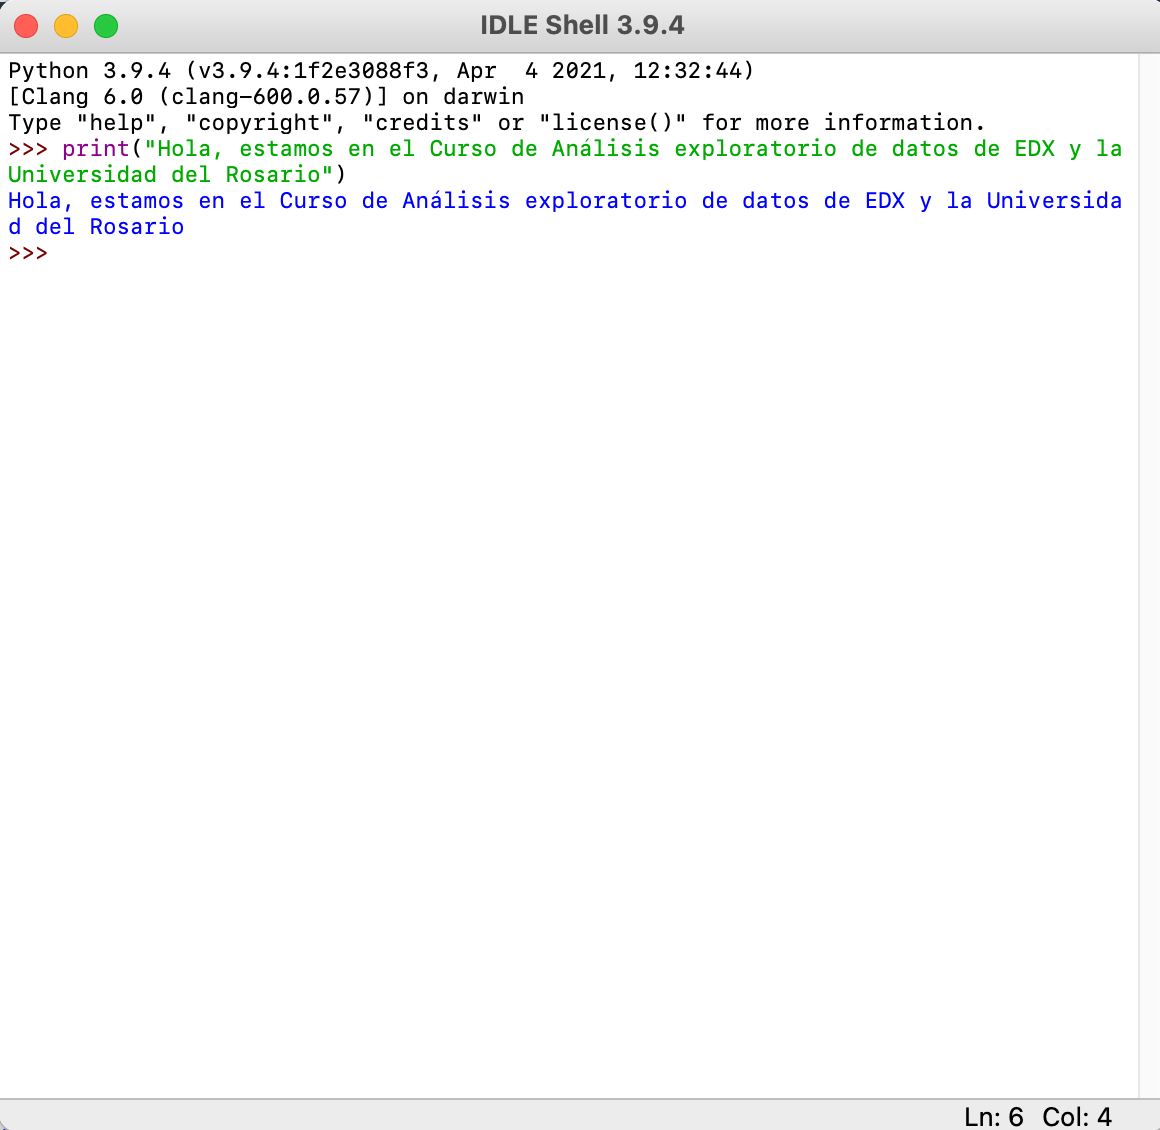
\includegraphics [width =0.55\textwidth]{IDEPY.png}
        \end{figure}
    \end{multicols}
\end{frame}

%% ---------------------------------------------------------------------------

\begin{frame}[fragile] 
    \frametitle{Uso online del Jupyter Notebook} 
    En caso de no querer descargar el Jupyter Notebook, es posible usarlo en el navegador (online) a través del siguiente link: {\color{blue}\url{https://jupyter.org/try}}
        \begin{figure}[H]
            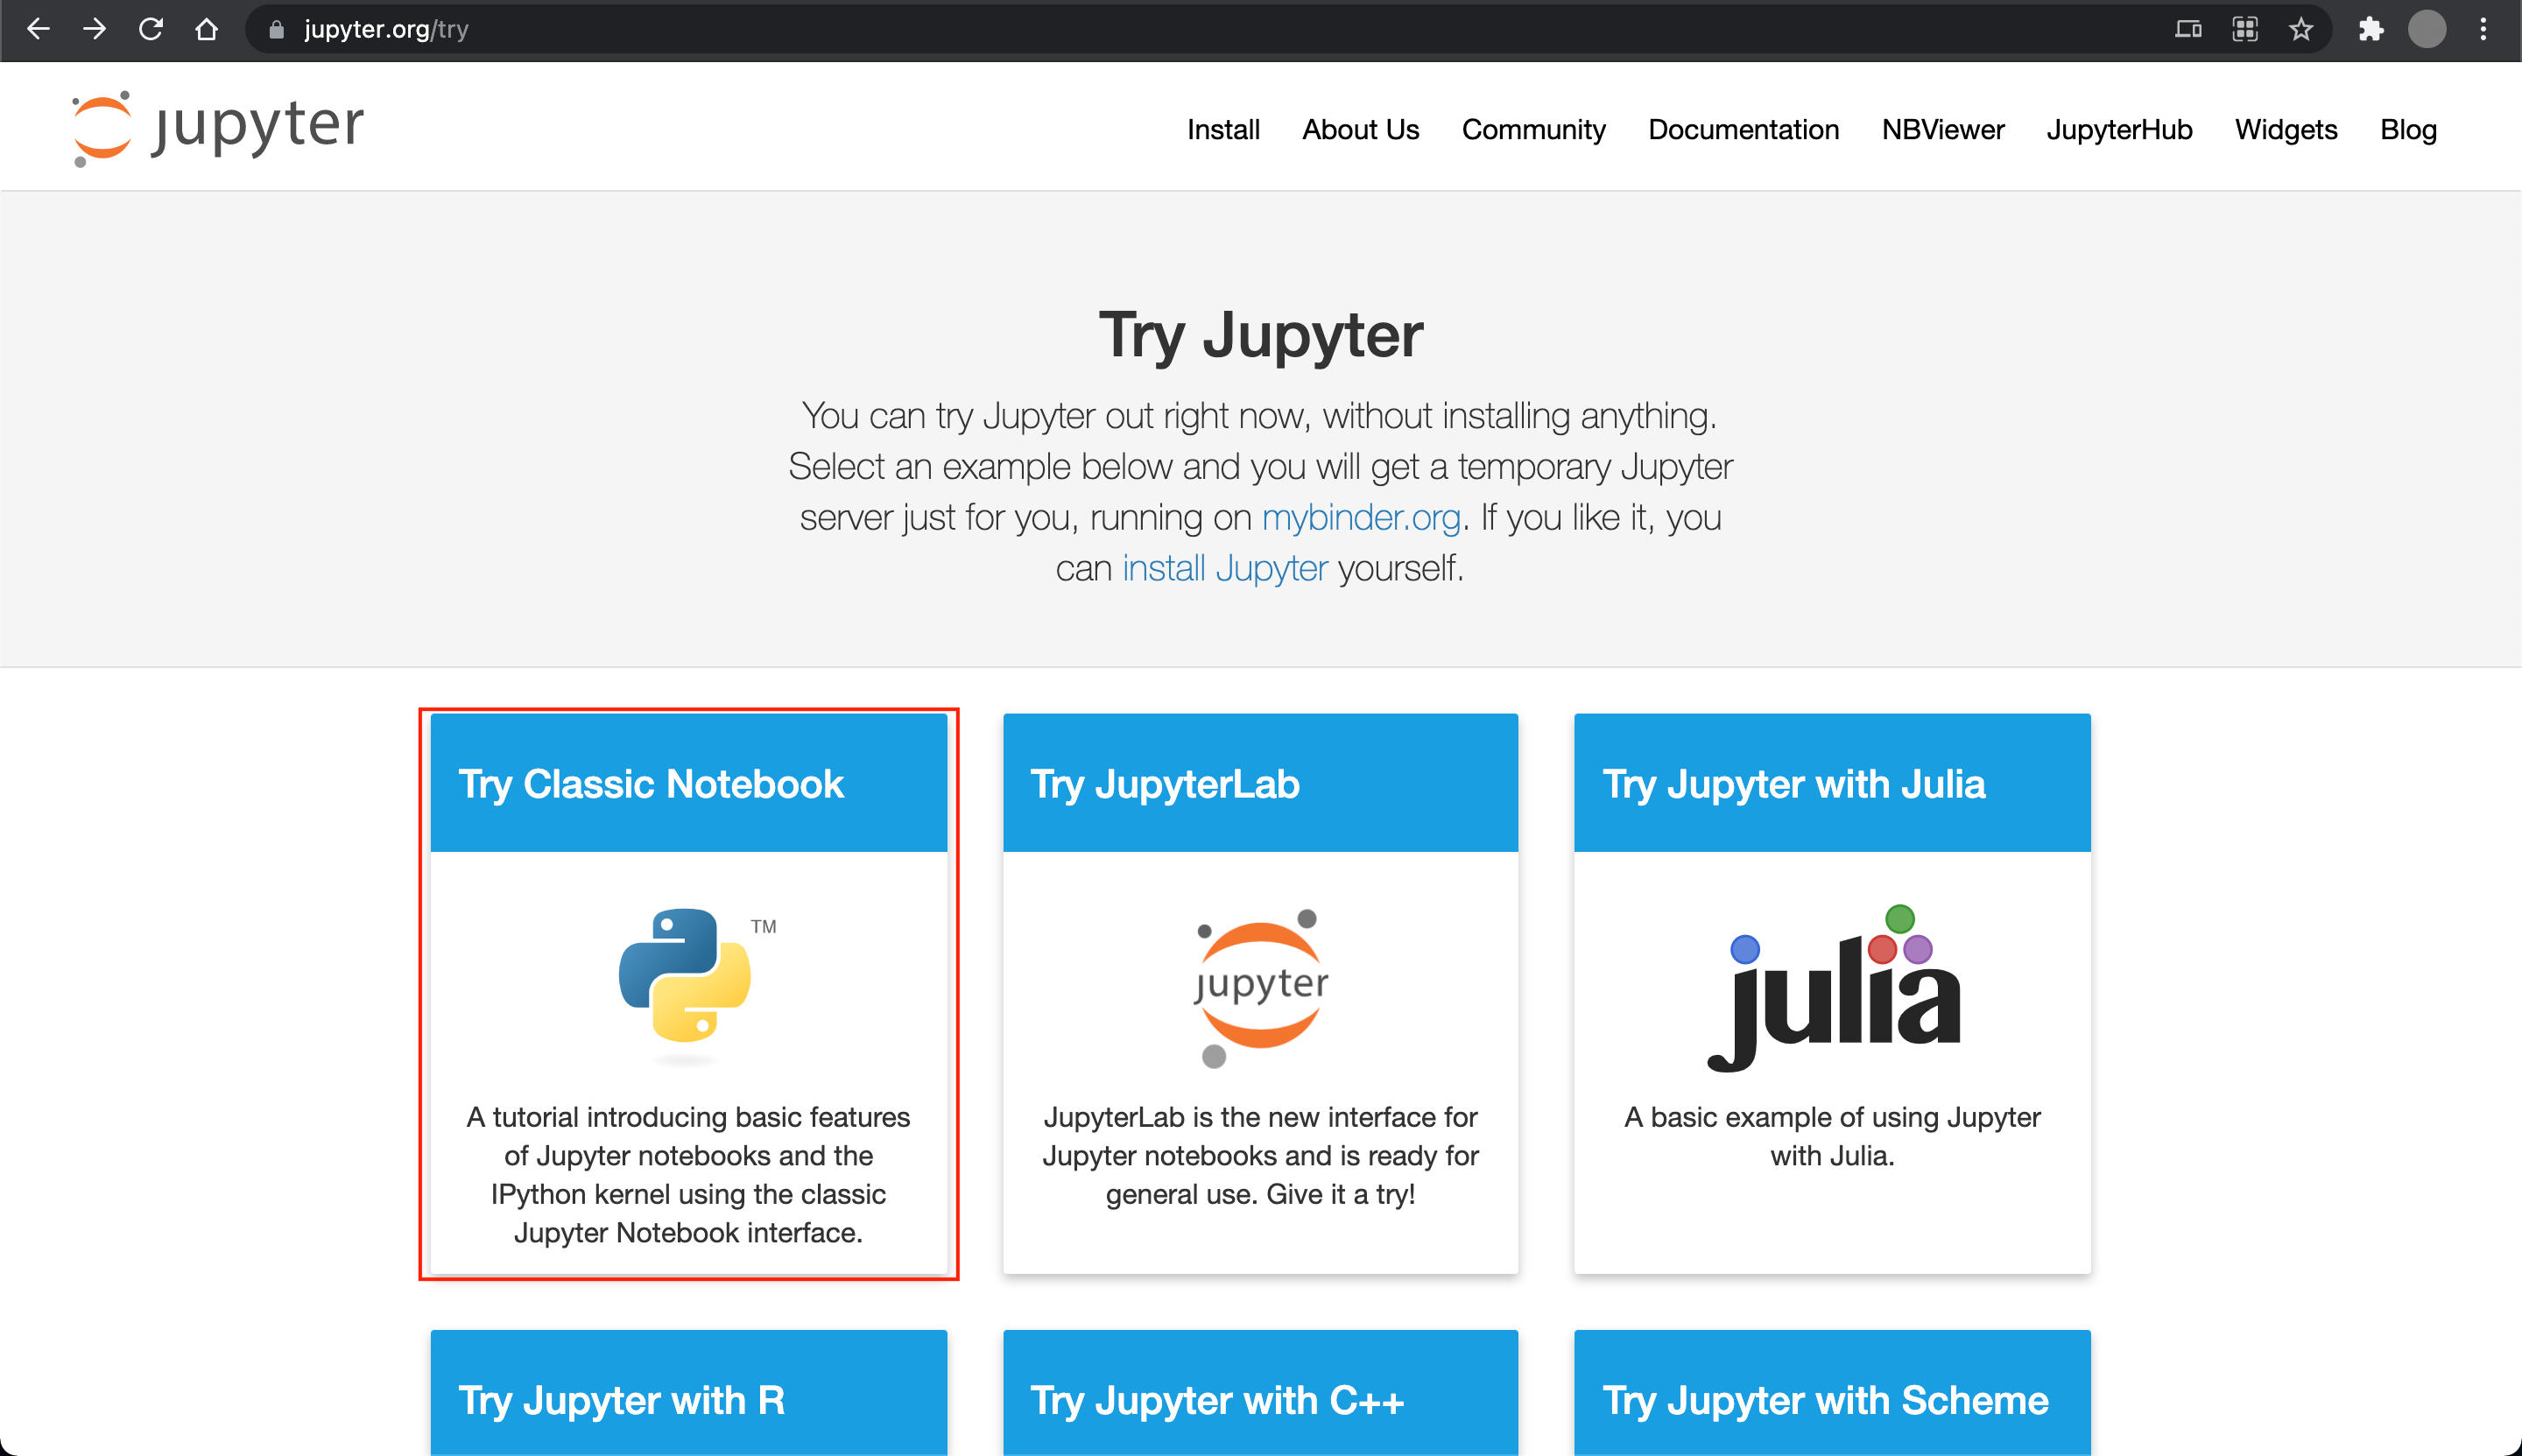
\includegraphics [width =0.5\textwidth]{JPONLINE.png}
        \end{figure}
    {\small Como se puede observar en este sitio web, el Jupyter Notebook no funciona únicamente con Python, sino con otros lenguajes de programación, entre estos R. Esta opcion se usará más adelante, por ahora se hará con Python.}
\end{frame}

%% ---------------------------------------------------------------------------

\begin{frame}[fragile] 
    \frametitle{Interfaz del Jupyter Notebook} 
    {\small El Jupyter Notebook instalado a través de anaconda, así como el usado de manera online, consisten en una página en el navegador (cualquiera: chrome, Mozilla o los de Microsoft), tal como se ve en la imagen:}
        \begin{figure}[H]
            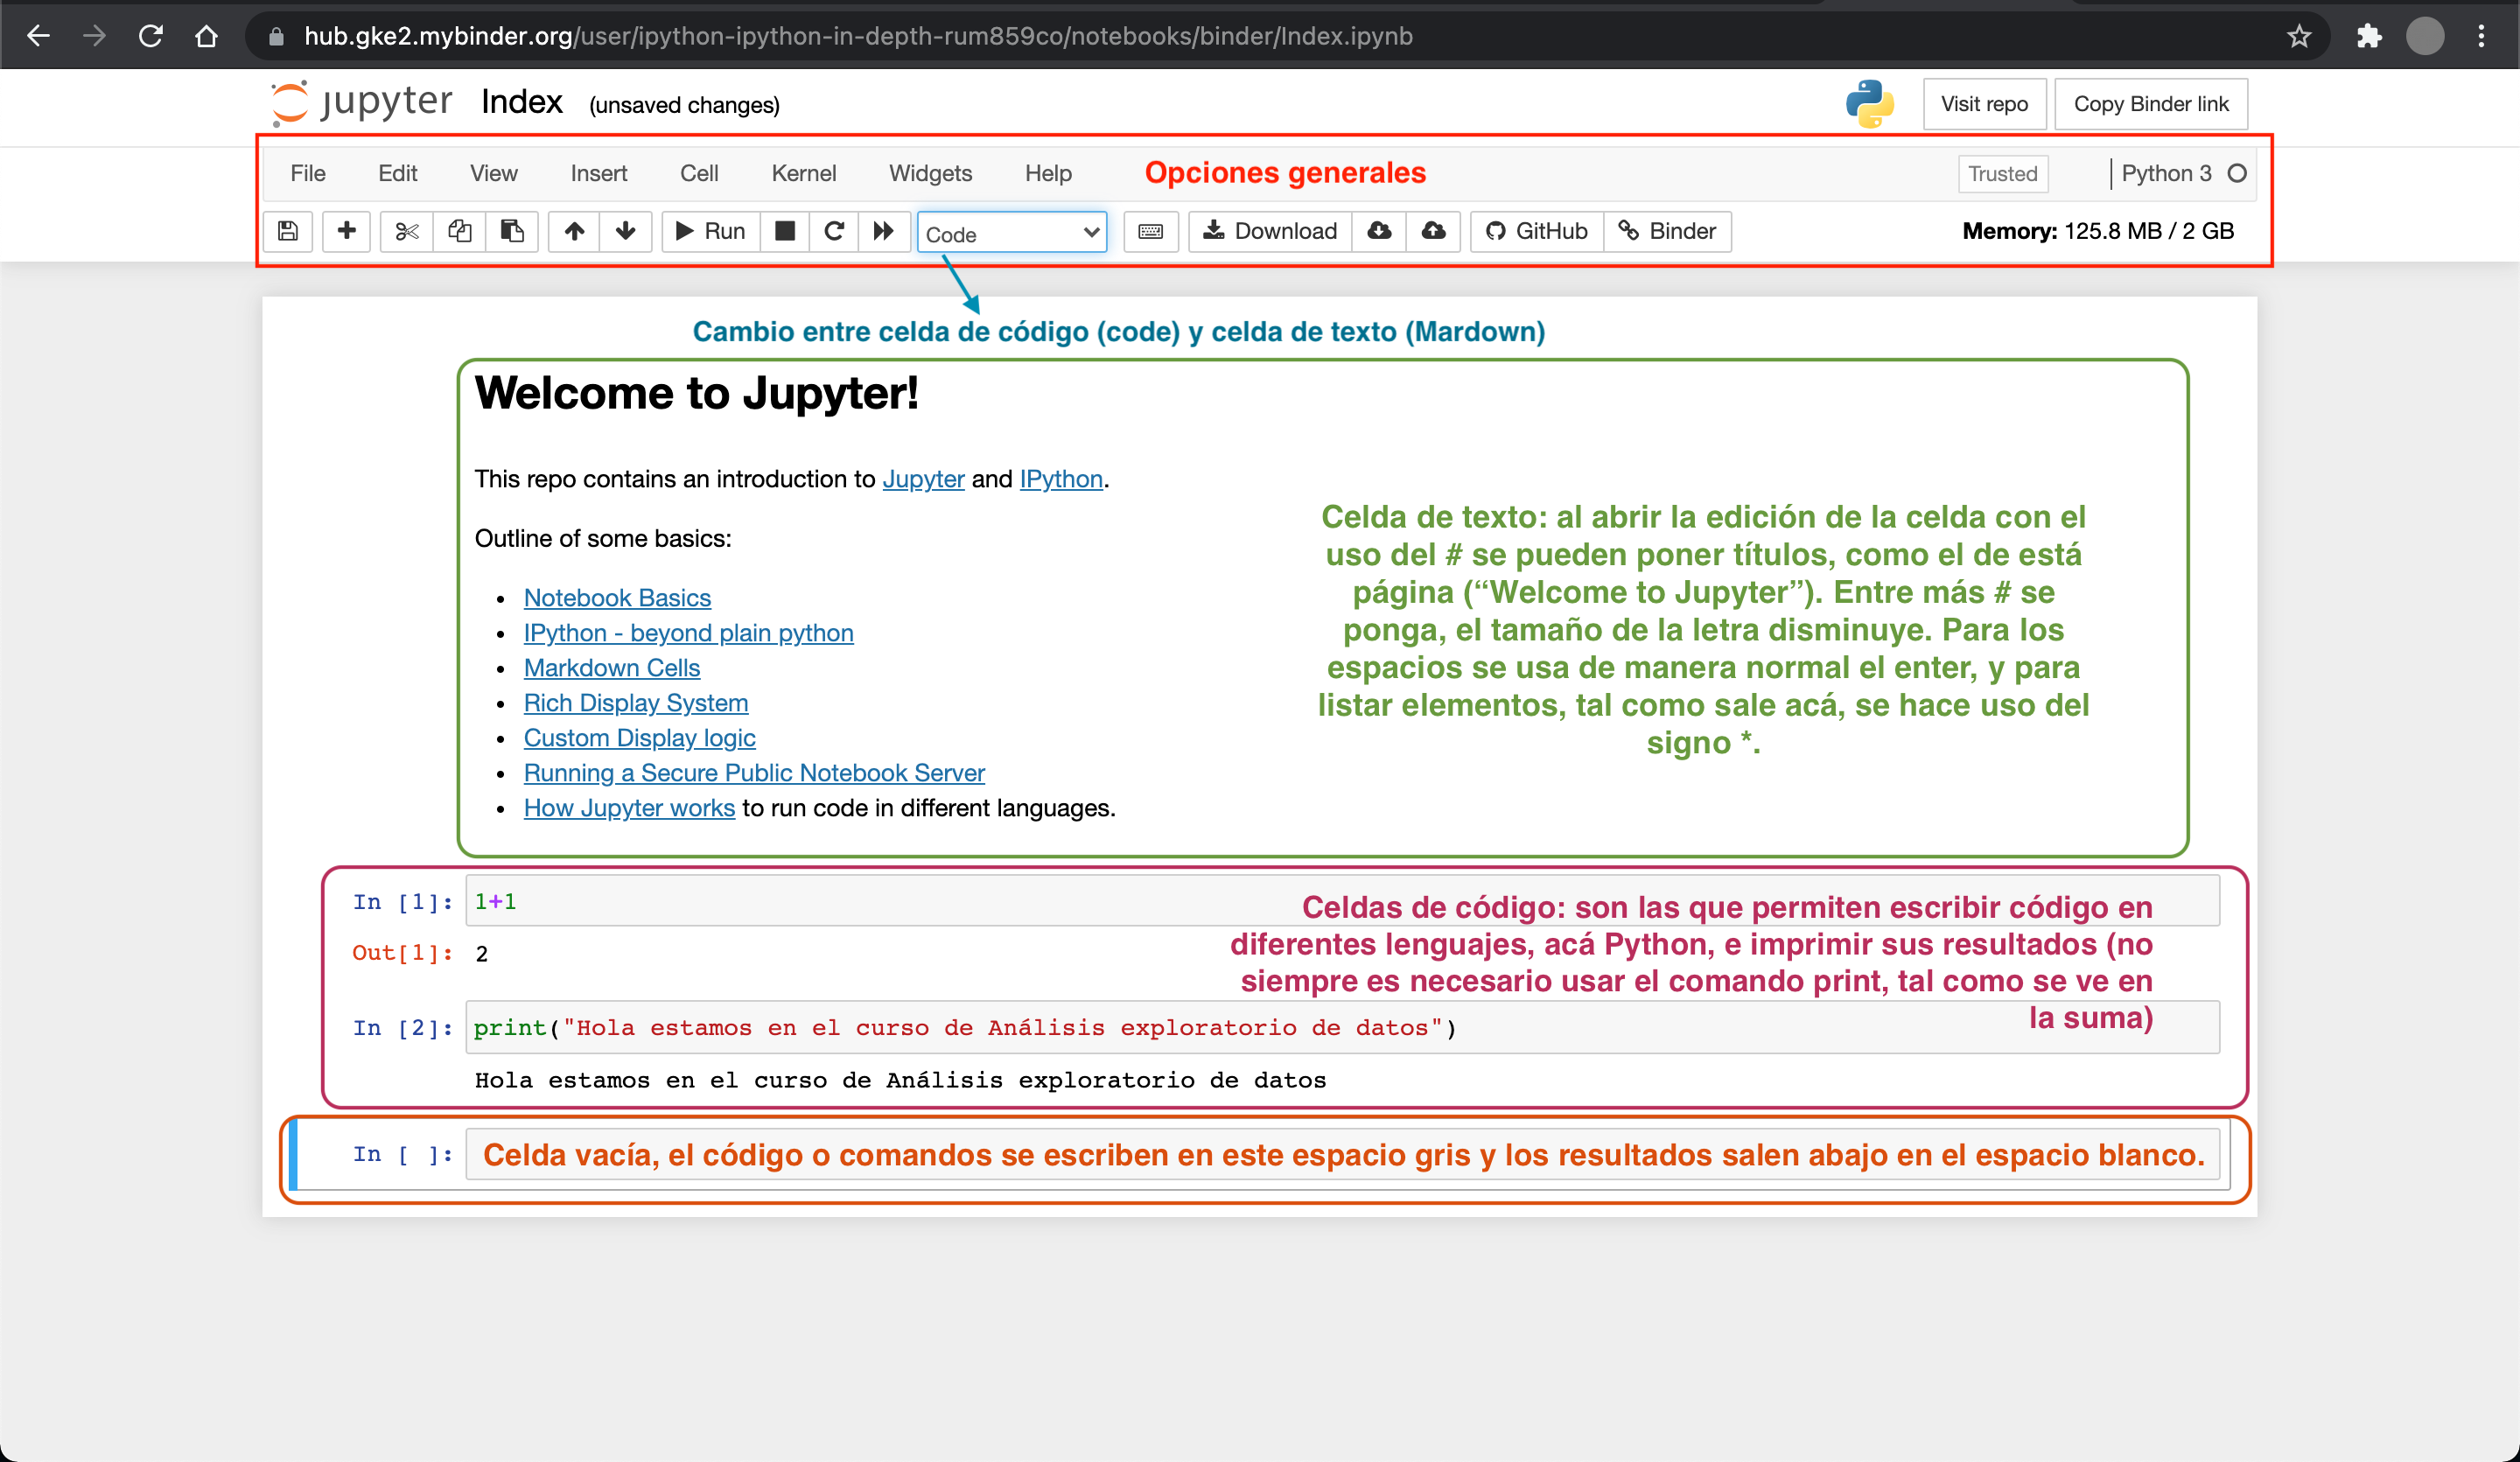
\includegraphics [width =0.85\textwidth]{InterfazJPN.png}
        \end{figure}
\end{frame}

%% ---------------------------------------------------------------------------
\section{Interfaz de R y R-Studio}

\begin{frame}[fragile] 
    \frametitle{Interfaz de R (IDE original)}
    \begin{multicols}{2}
        \begin{center}
        {\color{brown}{\small 
        Tal como el IDE original de Python, el de R es sencillo, funciona como una consola o terminal de código, en la cual, ante el uso del comando -print-, permite ver el resultado de los otros códigos utilizados, aunque no siempre es necesario hacer uso del print para que la consola imprima las salidas del código.}}
        \end{center}
        \begin{figure}[H]
            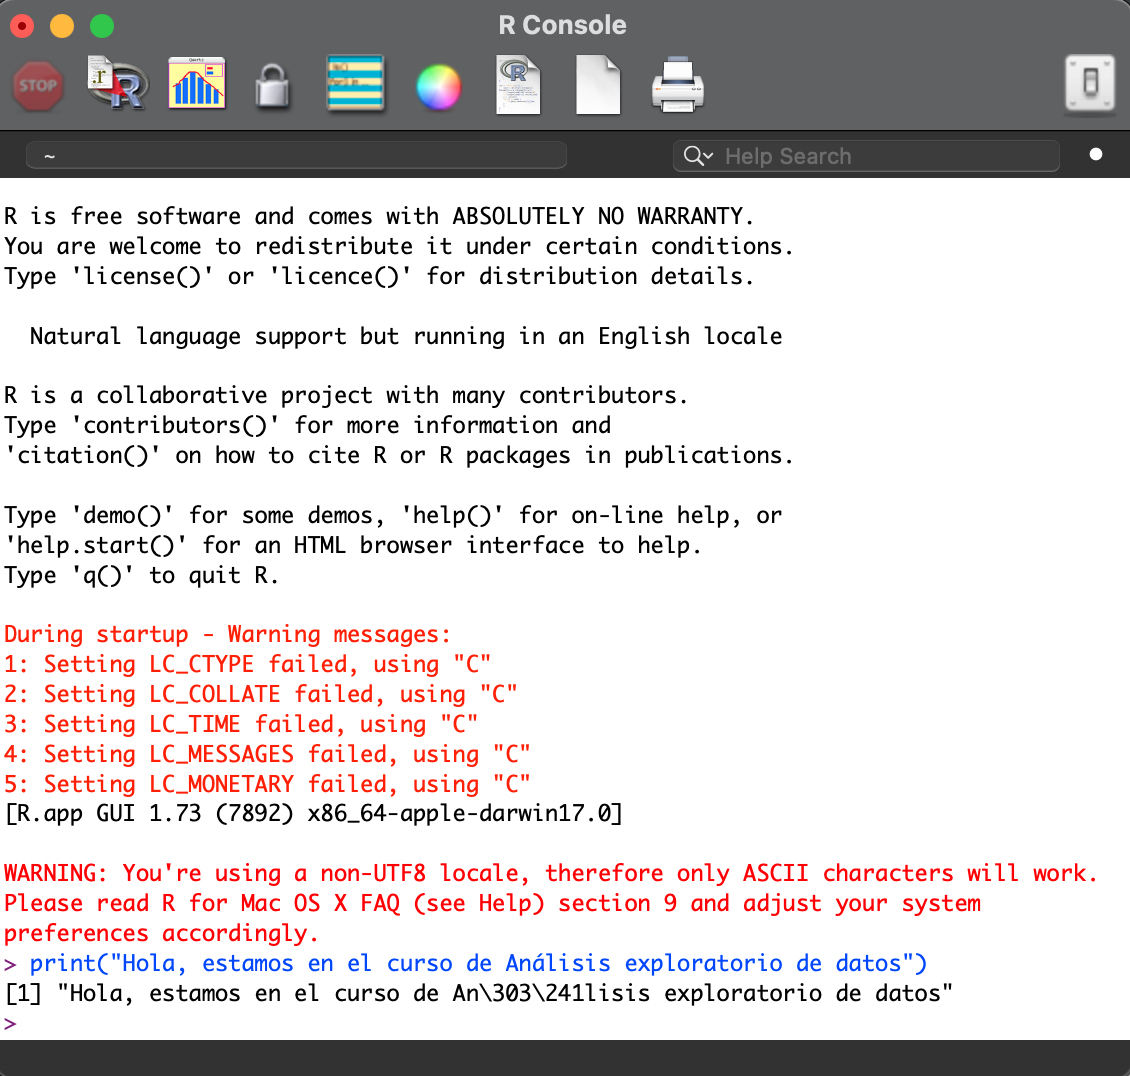
\includegraphics [width =0.55\textwidth]{IDER.png}
        \end{figure}
    \end{multicols}
\end{frame}

%% ---------------------------------------------------------------------------

\begin{frame}[fragile] 
    \frametitle{Interfaz de R-Studio Notebook} 
    {\small R-Studio funciona como un IDE muy amigable, instalado como un programa en el computador (aunque también funciona online) y que permite separar entre la consola, las bases de datos, la salida de resultados, gráficos y demás, como se ve en la imagen:}
        \begin{figure}[H]
            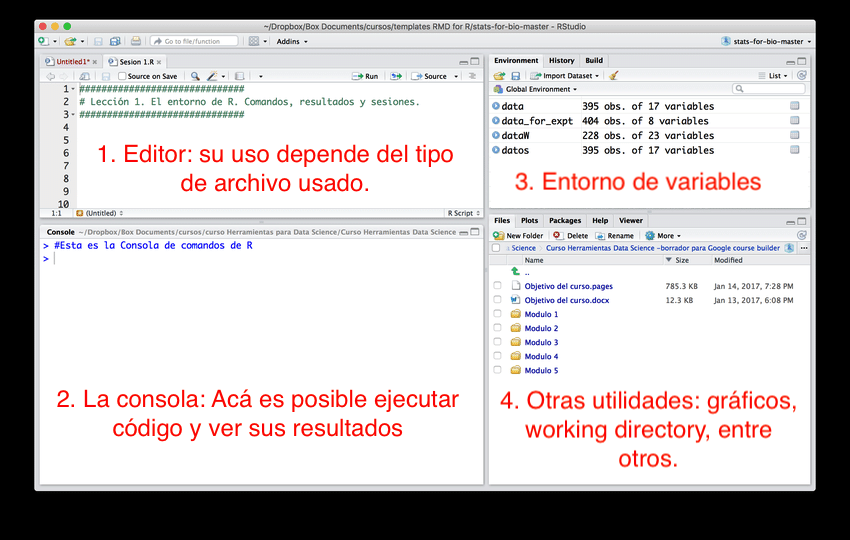
\includegraphics [width =0.8\textwidth]{Interfaz-de-RStudio.png}
        \end{figure}
\end{frame}

%% ---------------------------------------------------------------------------
\section{Bonus: Spyder (Anaconda, Python)}

\begin{frame}[fragile] 
    \frametitle{Interfaz de Spyder} 
        {\small El IDE Spyder instalado con el paquete Anaconda es muy parecido a R-Studio pero para programar en Python, permite separar la consola, las bases de datos, los resultados, gráficos y demás, como se ve en la imagen:}
        \begin{figure}[H]
            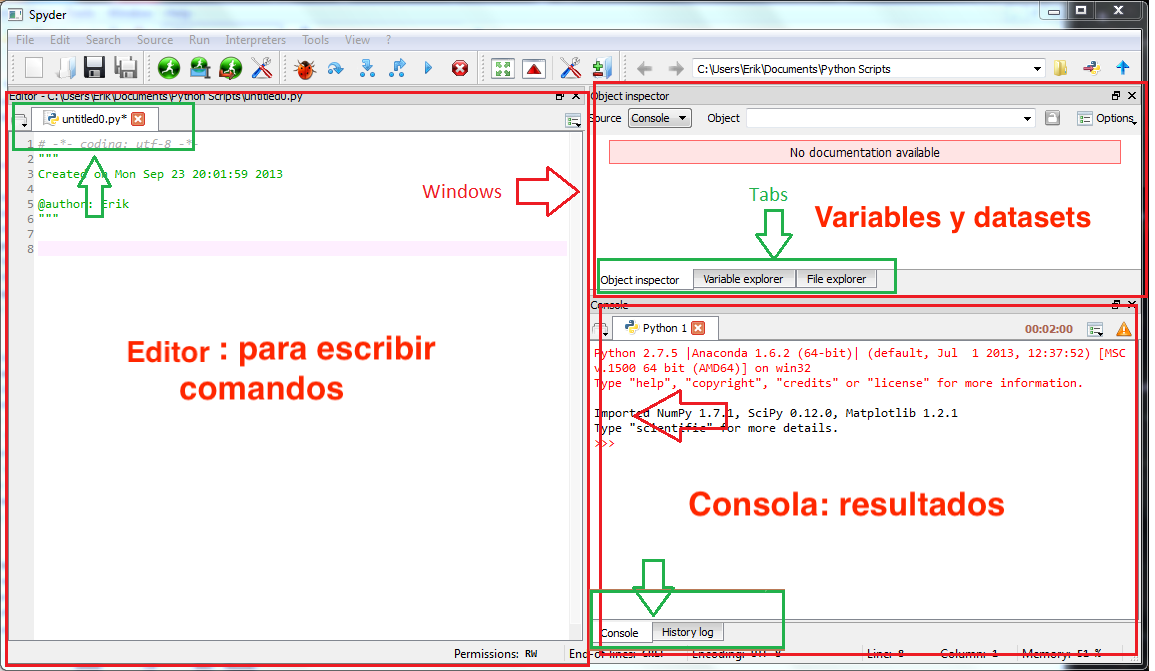
\includegraphics [width =0.85\textwidth]{openingscreencapture.png}
        \end{figure}
\end{frame}

%% ---------------------------------------------------------------------------

\end{document}